\section*{EXAMPLES}
In this section, three different examples are discussed. Their purpose is to numerically showcase that our method allows to adaptively refine the mesh to accurately solve an OCP, similarly to ~\cite{Patterson:OCAM:2015}, with the remarkable advantage of an increased computational efficiency for the final enhanced mesh without hindering the accuracy of the final solution.
%still within the specified tolerance.
In fact, by allowing to increase the degrees of the approximating polynomials independently for each state, our method effectively adopts to raise them carefully and in a tailored manner. This allows to reduce the overall number of variables of the resulting NLP, with clear benefits in terms of reduced CPU time, memory usage and reduced risk of being trapped by local minima.

Let us now direct our attention to the details. Each problem is transcribed in its initial NLP version by choosing $N = 20$ mesh intervals and by assigning a degree $\dki = 2$ everywhere, i.e. for all $i = 1, \dots, n_x$ and  $k = 1, \dots, N$. The mesh refinement algorithm is then applied with $d_{\min} = 2$, $d_{\max} = 8$ with a prescribed maximum allowable relative error $\epsilon = 1 \cdot 10^{-3}$.

It is worth observing that the $p_{n}h$ and $ph$ tags indicate our mesh refinement method and the one originally proposed by Patterson et al.~\cite{Patterson:OCAM:2015}, respectively.

It is also worth remarking that the final refined mesh for all the three presented examples (both in terms of number and size of $S_{k}$ intervals), turns out to be the same by rolling out both the $p_{n}h$ and the $ph$ approaches. This arises partly as a result that both algorithms share the last section (lines 9-14) of the \emph{Execution} pass in {\bf Algorithm~\ref{alg:step2}}. This means the generic $S_k$ interval is subdivided if and only if at least one state in the generic $S_k$ asks for it.

Each transcribed optimal control problem tested was coded in a scripting environment using the \text{MATLAB} interface to the open-source CasADi framework~\cite{casadi:MPC:2019}.
The CasADi suite can perform AD (Automatic Differentiation) on the code to compute gradients and Jacobians and provides building blocks to efficiently formulate and solve large-scale optimization problems. The back-end solver adopted is IPOPT~\cite{Biegler:CCE:2009} which implements an interior-point algorithm. All the associated NLPs are solved on a laptop with 2.30GHz Intel(R) Core(TM) i7-10875H CPU and 32 GB of RAM.



%%%%%%%%%%%%%%%%%%%%%%%%%%%%%%%%%%%%%%%%%%%%%%%%%%%%%%%%%%%%%%%%%%%%%%
\subsection*{Example 1: Van Der Pol}
The first optimal control problem considered is taken from reference~\cite{casadi:DOC:2018} and considers
driving a \emph{Van der Pol} oscillator to the origin. It can be expressed as follows
\begin{subequations}\label{eq:vanderpol}
	\begin{align}
	\underset{X \in \mathbb{R}^{2}, \, U \in \mathbb{R}}{\text{minimize}}\hspace{8mm}
	&J = \int_{0}^{T}(x_1^{2} + x_2^{2} + u^{2})\,dt  \label{eq:vancost}\\
	\text{subject to} \hspace{8mm} 
	&\dot{x}_1 = (1 - x_2^{2})x_{1} - x_2 + u \hspace{5mm} t \in[0,T] \label{eq:vandyn1}\\
	& \dot{x}_2 = x_1 \hspace{28.5mm} t \in[0,T] \label{eq:vandyn2}\\
	& -1  \leq u \leq 1,  \hspace{20mm} t \in[0,T] \label{eq:vanpath1}\\
	& x_2 \geq -0.25,  \hspace{21.5mm} t \in[0,T] \label{eq:vanpath2}\\
	 x_1(0) &= 0, \hspace{2mm} x_2(0) = 1, \label{eq:initial1}		
	%& x_2(0) = 1, \label{eq:intial2}		
	\end{align}
\end{subequations}
where $T = 10$ s, $x_1$ and $x_2$ are the two state components (hence $X(t) = [x_1(t), x_2(t)]\in \bbR^2$), $u\in\bbR$ indicates the control, and the dynamics constraints and the initial conditions are shown explicitly for each state component. Clearly, $\dot{X}(t) = [\dot{x}_1(t), \dot{x}_2(t)]$.

In Figs.~\ref{fig:pnh1vanderpol}--\ref{fig:pnh2vanderpol} (top panels) the final degrees of the first ($x_1$) and the second ($x_2$) state components, respectively, are shown. Here, the blue line is the outcome of the $\pnh$-mesh refinement algorithm whereas the green line is the result of the $ph$-one. With respect to the red line, which represents the initial degree, each method increases the degrees of the polynomials approximating the states. It is worth noting that the green line is the same for both figures, meaning that, according to the $ph$ logic, all the states share the same (maximum) polynomial order in the same interval $S_k$. Instead, the blue lines are different, meaning that each state has reached an independent degree for its polynomial approximation.
Furthermore, with respect to the initial $S_k$ steps delimited by the dashed gray lines, the more packed green and blue markers of the final solutions reveal where the $h$-strategy was adopted, thus producing a finer mesh.

In Figs.~\ref{fig:pnh1vanderpol}--\ref{fig:pnh2vanderpol} (bottom panels) the state profiles obtained with the $\pnh$ final mesh are shown. Here, the dashed gray lines delimit the \emph{final} mesh intervals. In particular, the nodal values are shown in blue, whereas the collocation points are plotted in red. These figures clearly show that the $\pnh$-adaptive mesh refinement method increases the polynomial order (more collocation points) and increases the mesh density (more mesh points) selectively for each state only where it is needed (higher gradient).
\begin{figure}[t]
	\centering
	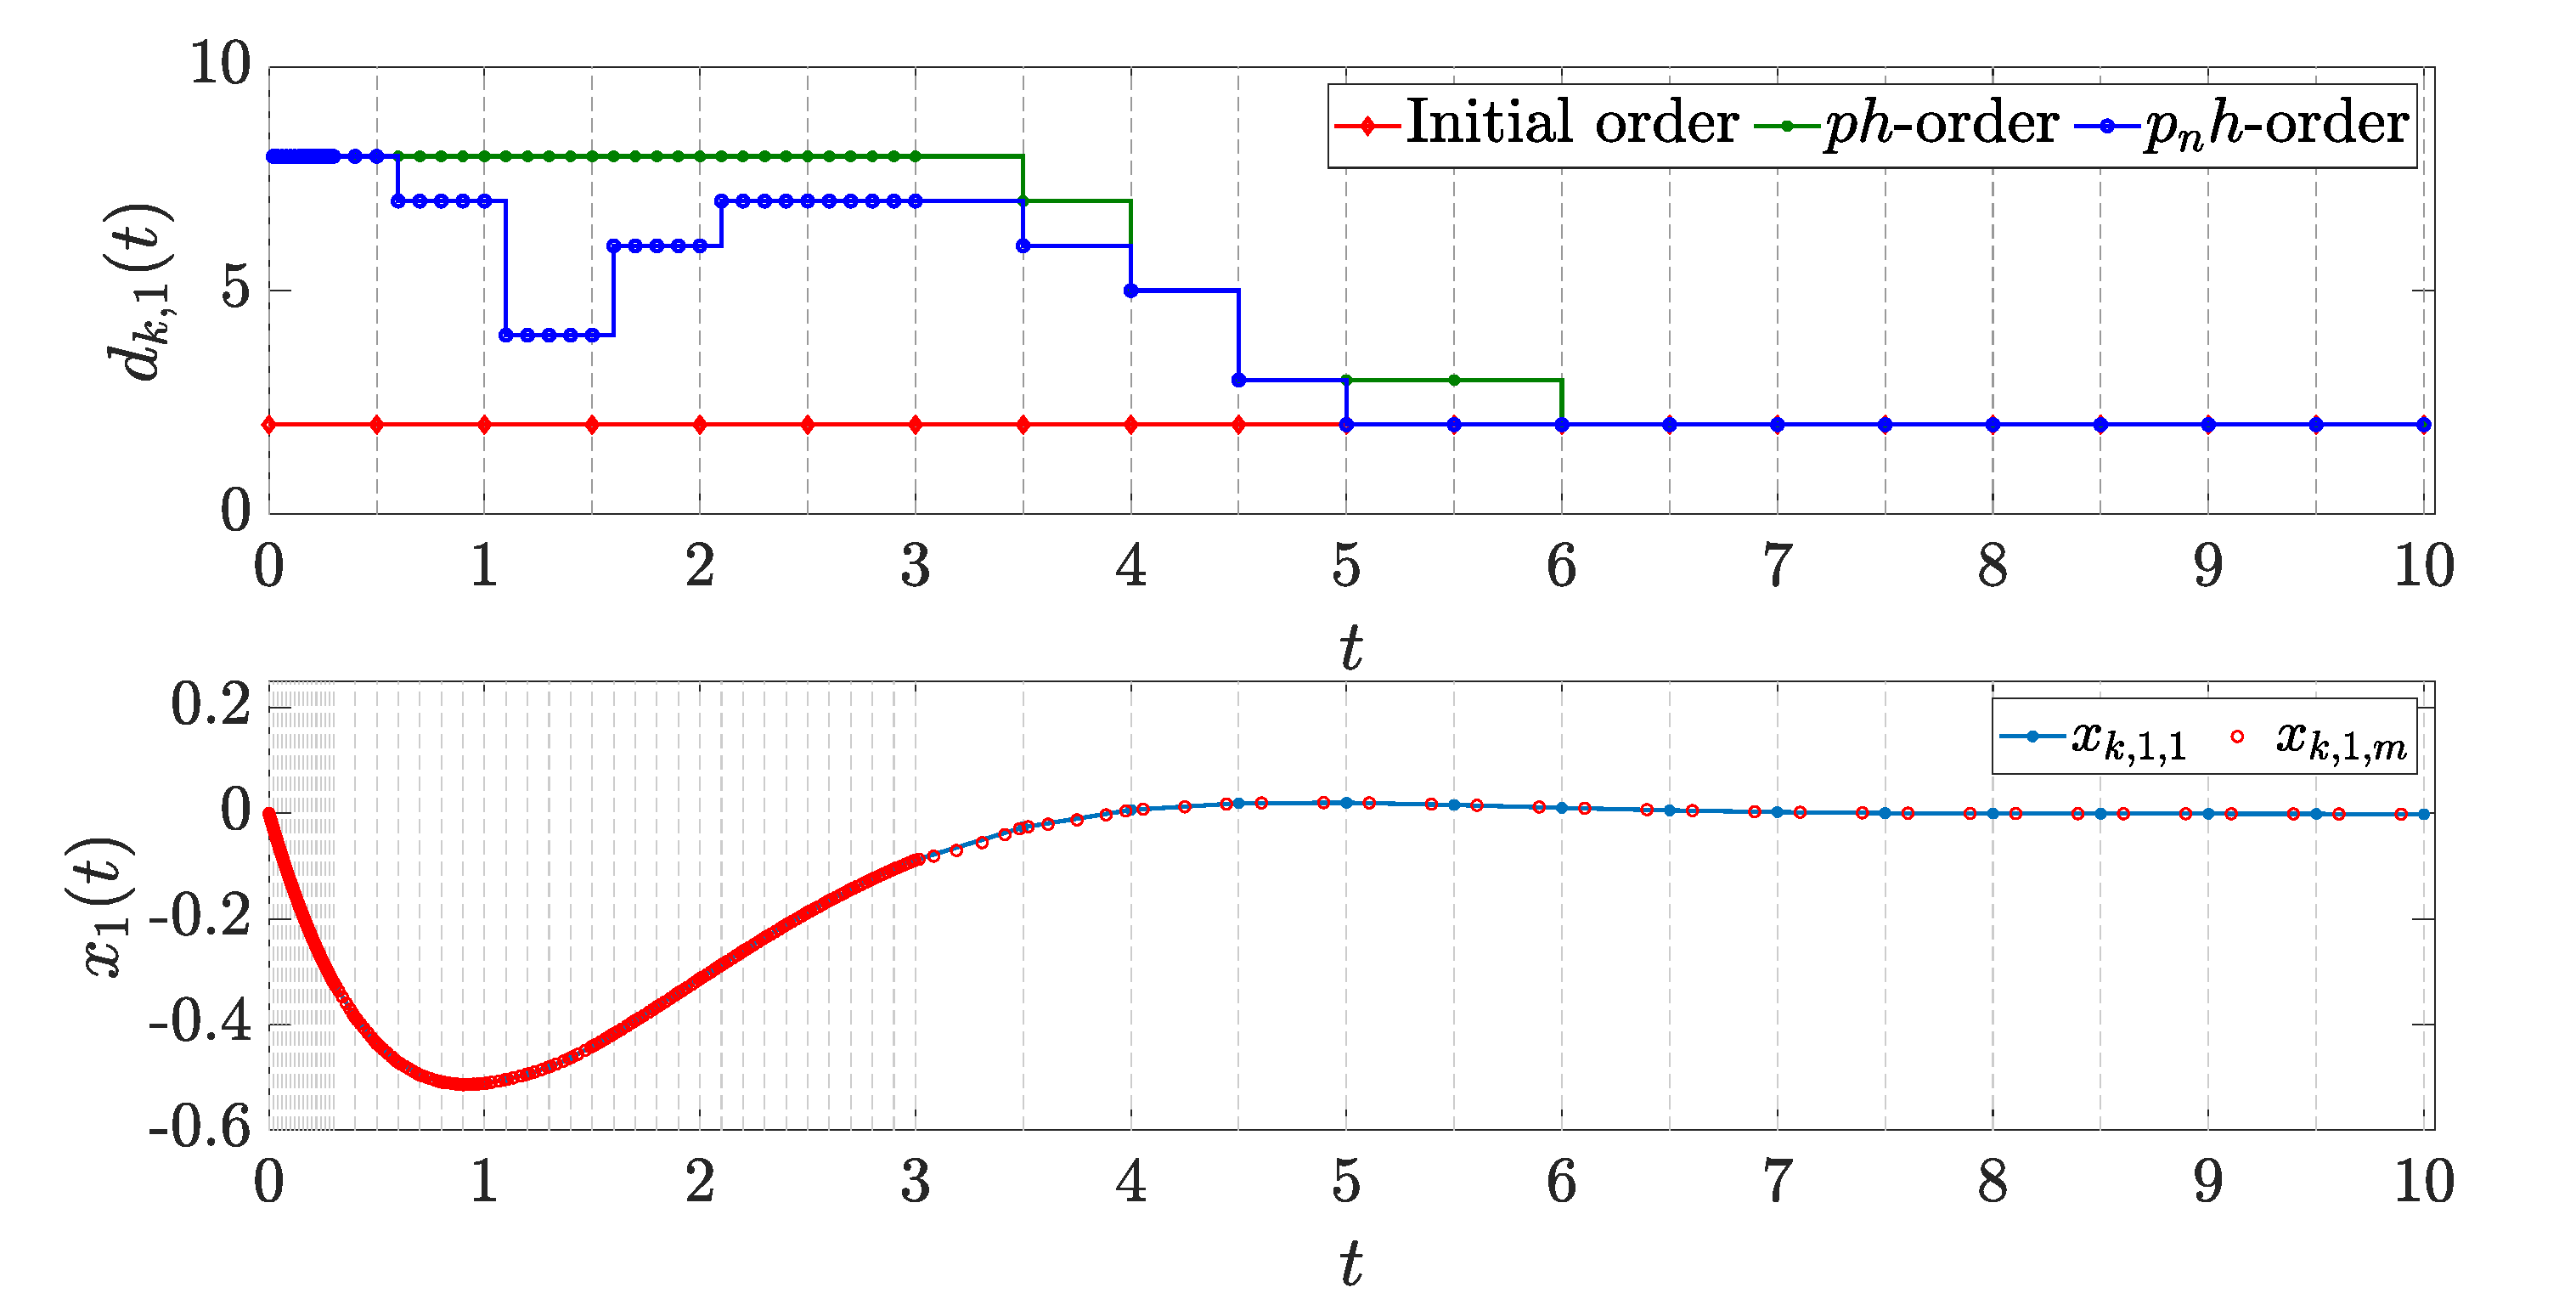
\includegraphics[trim={1cm 0.1cm 2cm 0.5cm},clip,width=1\columnwidth]{Img/pnh1_vanderpol1}
	\caption{EXAMPLE 1:  (TOP) POLYNOMIAL DEGREE OF $x_{1}$ FOR THE INITIAL MESH (RED) FOR $\pnh$ ALGORITHM (BLUE) AND FOR $ph$ ALGORITHM (GREEN), (BOTTOM)
	OPTIMAL $x_1$ PROFILE OBTAINED WITH $\pnh$.}
	\label{fig:pnh1vanderpol}
\end{figure}
\begin{figure}[t]
	\centering
	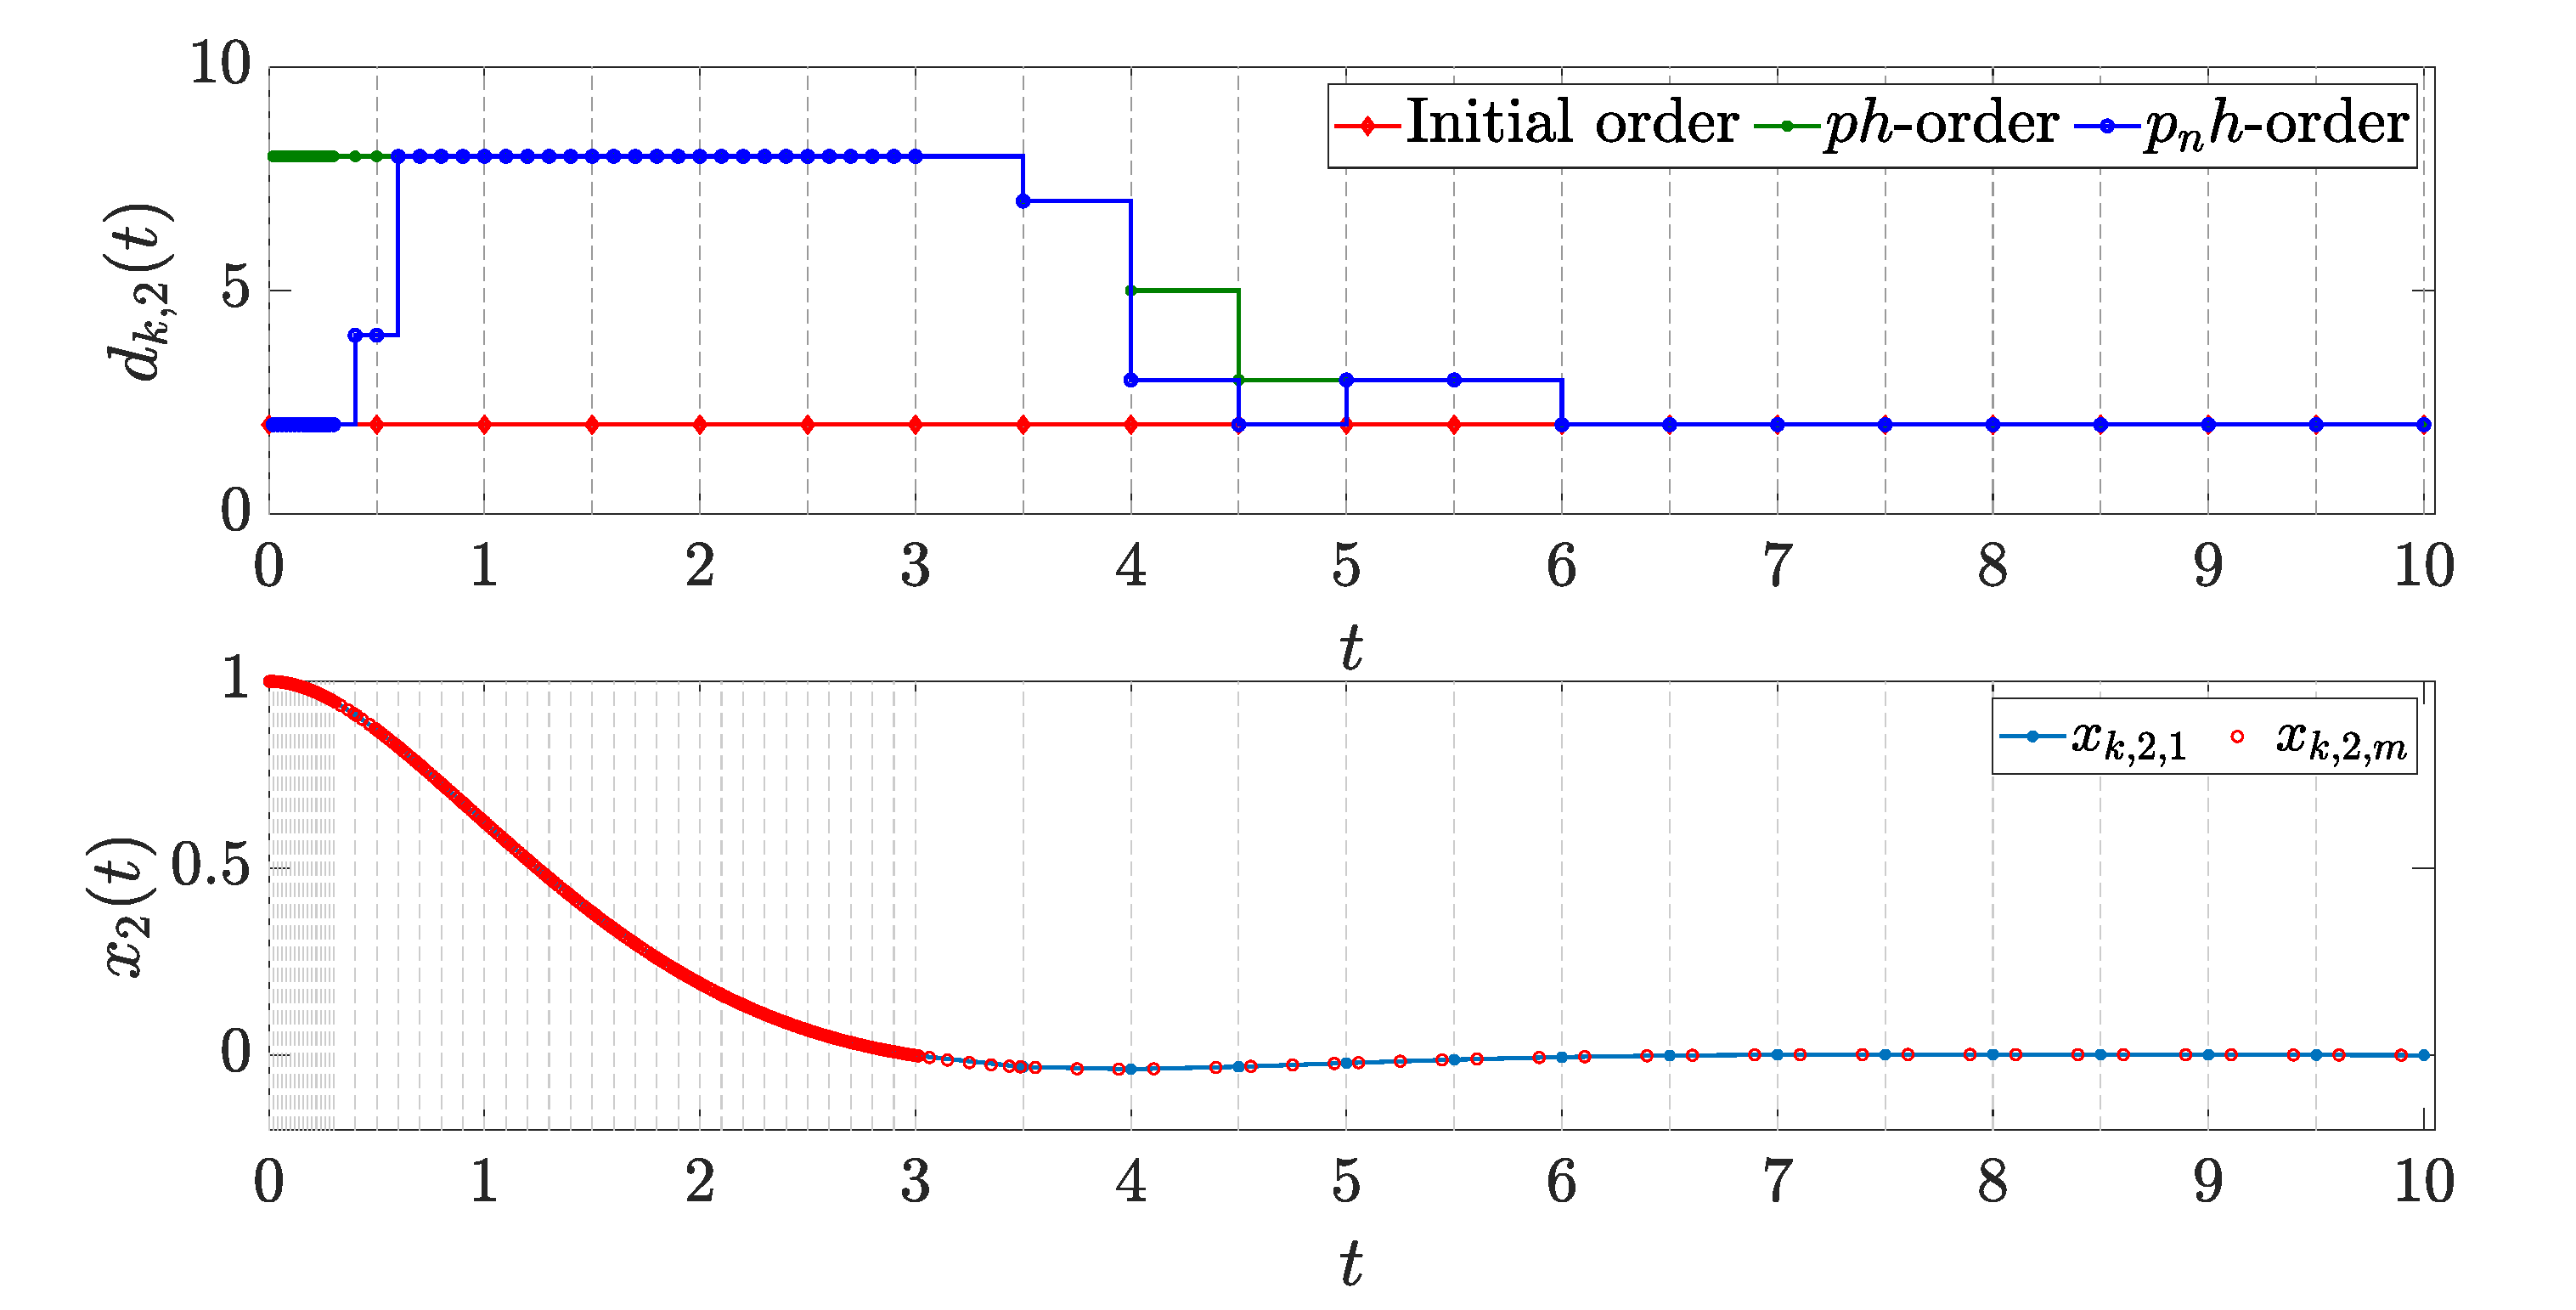
\includegraphics[trim={1cm 0.1cm 2cm 0.5cm},clip,width=1\columnwidth]{Img/pnh2_vanderpol2}
	\caption{EXAMPLE 1: (TOP) POLYNOMIAL DEGREE OF $x_{2}$ FOR THE INITIAL MESH (RED) FOR $\pnh$ ALGORITHM (BLUE) AND FOR $ph$ ALGORITHM (GREEN) (TOP), (BOTTOM)
	OPTIMAL $x_1$ PROFILE OBTAINED WITH  $\pnh$.}
	\label{fig:pnh2vanderpol}
\end{figure}
The advantages of the $\pnh$ method with respect to the $ph$ one are shown in Table~\ref{tab:tablevanderpol}. Here, the \emph{Mesh} column indicates the type of discretization mesh. In particular, \emph{Initial} refers to the mesh of the initial problem, whereas $ph$ and $\pnh$ refer to the final meshes produced by applying the methods in~\cite{Patterson:OCAM:2015} and ours, respectively. It is worth remarking that both of them comply with the prescribed tolerance $\epsilon=10^{-3}$. Furthermore, \emph{Vars} indicates the number of variables of the NLP associated to the transcribed OCP. Then, \emph{Soln. time} indicates the time to solution of the optimal control problem with the refined mesh. Finally, \emph{Iter} refers to the number of algorithm iterations needed to reach the prescribed accuracy, whereas \emph{Tot.\,time} is the total CPU time elapsed to reach the imposed convergence criterion. It is worth remarking that it includes the necessary time to build and solve all the \emph{Iter} $+1$ number of successive NLP problems and the time spent by the application of a number of \emph{Iter} mesh refinement algorithms. Finally, $e_{\max}$  is the maximum of the local error $\ekij$, hence
\begin{equation}
e_\text{max}= \max\limits_{\substack{j = 1, \dots, \dkip \\ i = 1, \dots, n_x \\ k = 1, \dots, N}} (\ekij)
\end{equation}
\begin{table}[t]
	\caption{EXAMPLE 1: MESH REFINEMENT RESULTS FOR THE THREE DIFFERENT TYPE OF MESH (INITIAL MESH, $ph$ FINAL MESH AND $\pnh$ FINAL MESH)}
	\begin{center}
		\label{tab:tablevanderpol}
		\begin{tabular}{c c c c c c c}
			& & \\ % put some space after the caption
			\hline
			\emph{Mesh} & \emph{Vars} & \emph{Soln. time} & \emph{Iter} & \emph{Tot. time} & $e_\text{max}$ \\
			\hline
			\emph{Initial} & 140 & 138 ms & / & / &  $3.7\cdot 10^{-2}$\\
			$ph$ & 918 & 500 ms & 4 & 23.1 s & $9.1\cdot 10^{-4}$ \\
			$\pnh$ & 769 & 400 ms & 4 & 19.0 s & $9.5\cdot 10^{-4}$ \\
			\hline
		\end{tabular}
	\end{center}
\end{table}
%%%%
\begin{figure}[t]
	\centering
	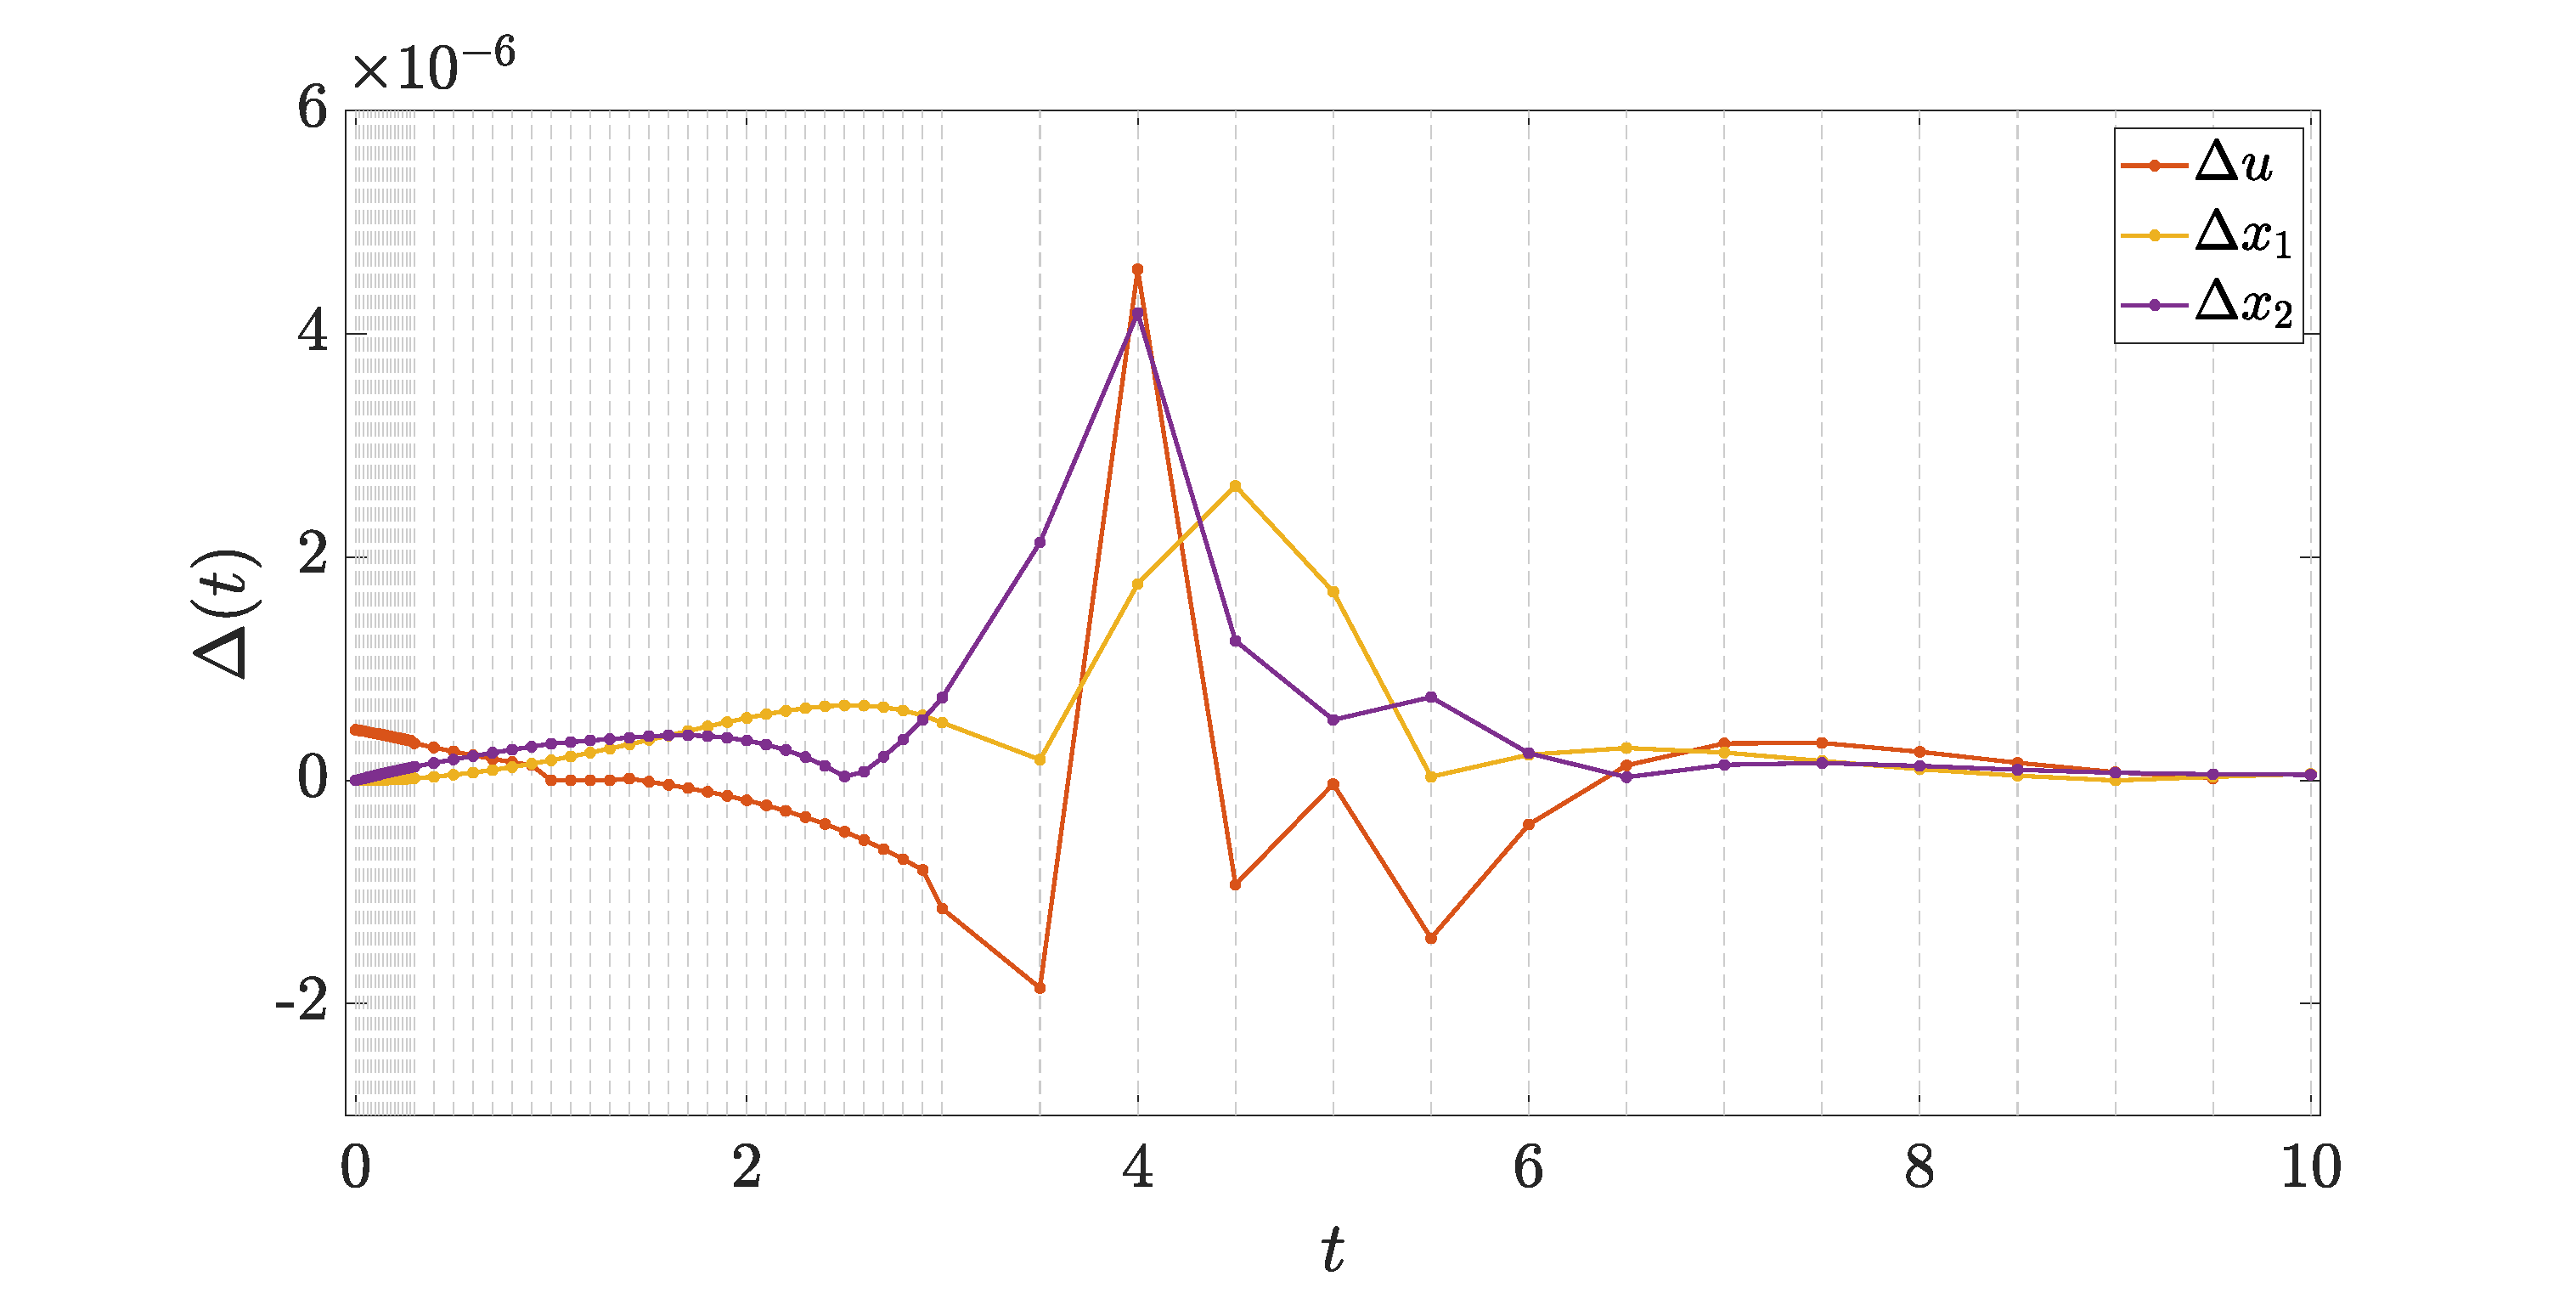
\includegraphics[trim={2cm 0.5cm 4cm 0.3cm},clip,width=1\columnwidth]{Img/delta_vanderpol}
	\caption{EXAMPLE 1: NODAL DIFFERENCES BETWEEN $\pnh$ AND $ph$ FINAL SOLUTIONS}
	\label{fig:deltavanderpol}
\end{figure}
It is worth stressing that the solution associated to a \emph{coarser} discretization, produced by the $\pnh$ method, still complies with the given tolerance $\epsilon$ while leading to an NLP with sensibly fewer variables than the $ph$ algorithm.
Hence, as a general benefit, the final NLP obtained from our method requires a reduced computational cost and a shorter CPU time.
Furthermore, considering that $ph$ and $\pnh$ have the same final mesh in terms of $S_k$ number and size, these two solution can be compared at the nodal values.
In Figure~\ref{fig:deltavanderpol}, the deviations between the $\pnh$ and $ph$ final optimal solutions, are shown.
Given that both the states $x_1$ and $x_2$ and the control $u$ are in the order of $10^{0}$, the deviations $\Delta(\cdot)$ are absolutely negligible and the two solutions are practically the same.
%%%%%%%%%%%%%%%%%%%%%%%%%%%%%%%%%%%%%%%%%%%%%%%%%%%%%%%%%%%%%%%%%%%%%%
\subsection*{Example 2: Rolling (Not Falling) Disk}
The second optimal control problem consists in driving a rolling (not falling) disk on an horizontal $x$-$y$ plane from an initial position to a final one, while minimizing the control action. This can be expressed as follows
\begin{subequations}\label{eq:disk}
	\begin{align}
	\underset{X \in \mathbb{R}^{6}, \, U \in \mathbb{R}^{2}}{\text{minimize}}\hspace{8mm}
	&J = \int_{0}^{T}(u_{1}^{2} +  u_{2}^{2})\,dt  \label{eq:diskcost}\\
	\text{subject to} \hspace{8mm}
	& \dot{x}_1 = \rho x_6  \cos(x_3) \hspace{10mm} t \in[0,T] \label{eq:diskdyn1}\\
	& \dot{x}_2 = \rho x_6  \sin(x_3)\hspace{10.5mm} t \in[0,T] \label{eq:diskdyn2}\\
	& \dot{x}_3 = x_5\hspace{23mm} t \in[0,T] \label{eq:diskdyn3}\\
	& \dot{x}_4 = x_6\hspace{23mm} t \in[0,T] \label{eq:diskdyn4}\\
	& \dot{x}_5 = u_1/I_{\theta}\hspace{18.2mm} t \in[0,T] \label{eq:diskdyn5}\\
	& \dot{x}_6 = u_2/(I_{\phi} + m \rho^{2})\hspace{5.8mm} t \in[0,T] \label{eq:diskdyn6}\\
	& x_6 \geq 0  \hspace{24.5mm} t \in[0,T]\\
	&X(0) = [0, 0, \pi/2, 0, 0, 0]\\	
	 x_1(T) = 10,\hspace{2mm} &x_2(T) = 10, \hspace{2mm} x_3(T) = \pi/4, \label{eq:diskfinal1}		
	\end{align}
\end{subequations}
where $T = 10$ s, $m$ is mass of the disk, $\rho$ is the disk radius, $I_{\theta}$ is the diametral moment of inertia and
%respect to an axis that passes through the contact point between the disk and the plane and perpendicular to the latter; 
$I_{\phi}$ is the axial disk moment of inertia.
%respect to an axis that passes through the center of the disk and is parallel to the plane.
States $x_1$ and $x_2$ represent the trajectory of the contact point of the disk on the plane, $x_3$ is the heading angle measured with respect to
%as measured between the disk rolling direction and 
the $x$-axis and $x_4$ is the rolling angle. Then, $x_5$, $x_6$ are the steering and rolling speed, respectively.
The disk is controlled with two torques, $u_1$ for the steering action and $u_2$ for the rolling action. Starting at the origin ($x_1(0) = 0, \, x_2(0) = 0$) and heading along the $y$-axis ($x_3(0) = \pi/2$), the disk has to reach the final position described by
Eqn.~(\ref{eq:diskfinal1}). It is worth recalling that, for a more compact notation, $X = [x_1, x_2, x_3, x_4, x_5, x_6]$  and $U = [u_1, u_2]$.
\begin{figure}[t]
	\centering
	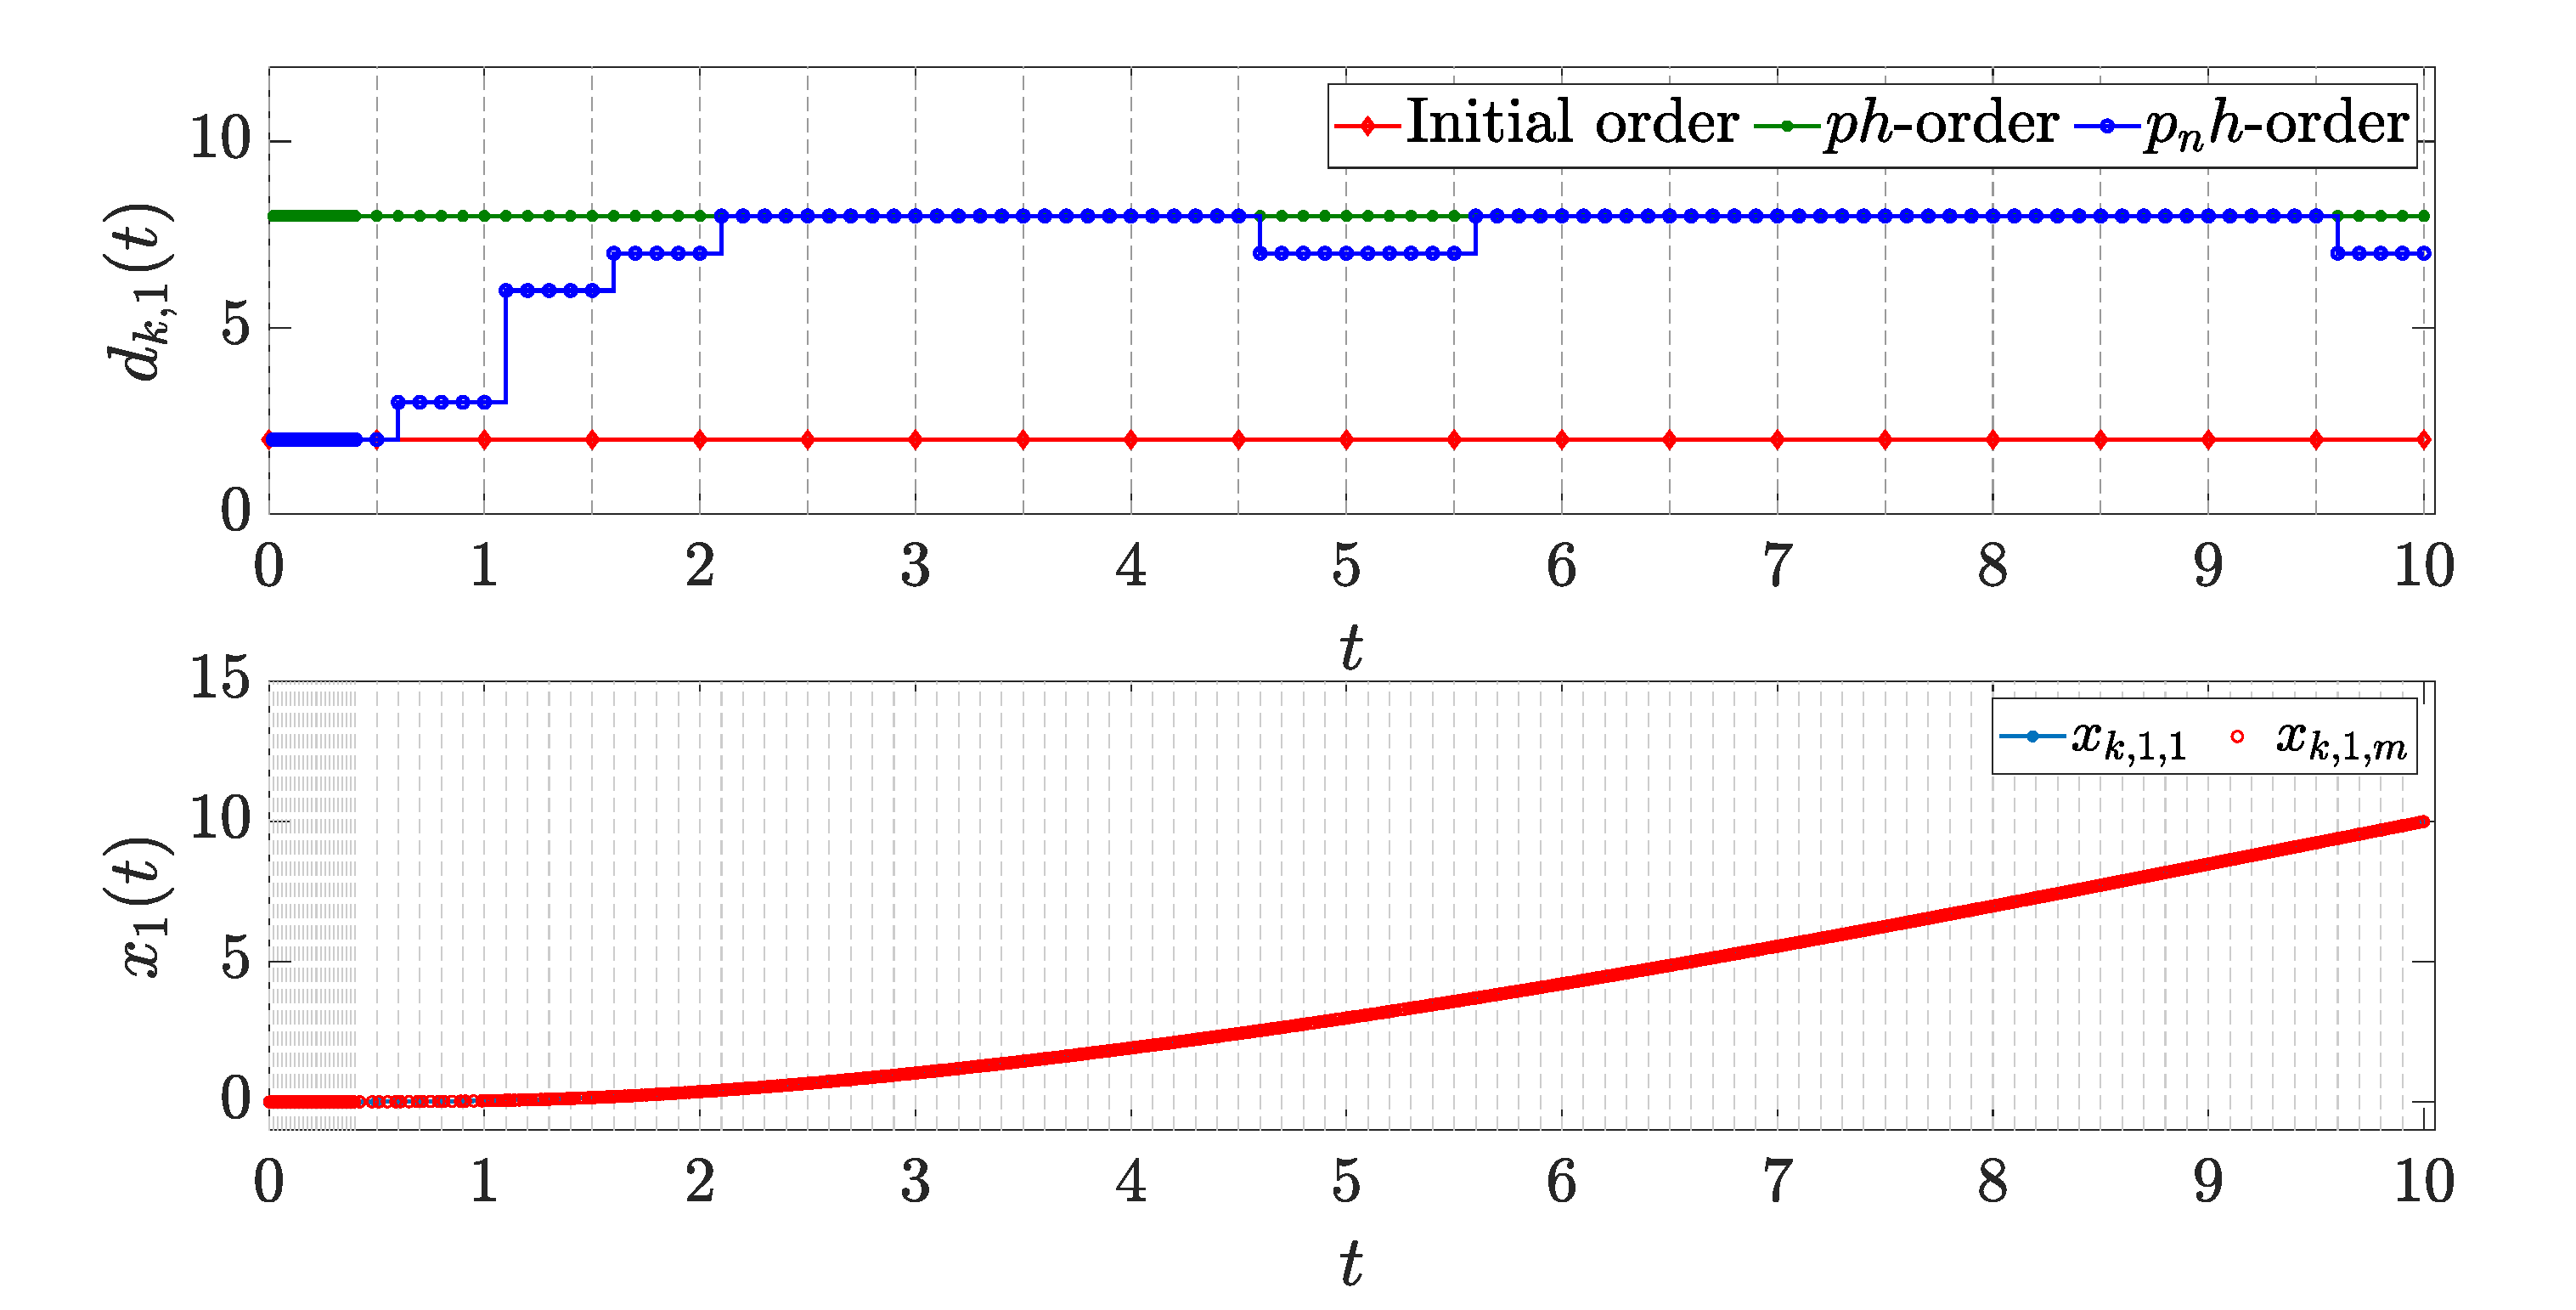
\includegraphics[trim={1cm 0.1cm 2cm 1.05cm},clip,width=1\columnwidth]{Img/pnh1_disk1}
	\caption{EXAMPLE 2: (TOP) POLYNOMIAL DEGREE OF FIRST STATE ($x_{1}$) FOR THE INITIAL MESH (RED) FOR $\pnh$ ALGORITHM (BLUE) AND FOR $ph$ ALGORITHM (GREEN), (BOTTOM)
		OPTIMAL $x_1$ PROFILE OBTAINED WITH $\pnh$.}
	\label{fig:pnh1disk}
\end{figure}
In Figs.~\ref{fig:pnh1disk}-\ref{fig:pnh2disk} (top panels) is shown, for the $\pnh$ algorithm and for the $ph$ one, the final degree of state $x_1$ (horizontal coordinate) and of state $x_3$ (heading angle), respectively.
With reference to Figure~\ref{fig:pnh1disk} (top panel), both $\pnh$ and $ph$ return for state $x_1$ almost the same polynomial degree for the whole time horizon. However, as evident from Figure~\ref{fig:pnh2disk} (top panel), for state $x_3$ the two algorithms provide very different polynomial degrees for most of the time horizon.
In particular, the green line always at $d_{\max}=8$ imply that in each mesh interval, there is at least one state (different from $x_3$, surely $x_1$) that requires that particular polynomial order. Instead, by applying the $\pnh$ method, each state is approximated with a polynomial degree that is \emph{just right}.
More in details, considering the solution in the range 6-9s, the state $x_1$ requires the maximum achievable order $d_\text{max} = 8$. This leads to an overkill in the approximation of the state $x_3$ with the same degree for the $ph$ method, while a lower degree as suggested by the $\pnh$ method is sufficient.

In Figs.~\ref{fig:pnh1disk}-\ref{fig:pnh2disk} (bottom panels) the optimal profile of $x_1$ and $x_3$ are shown. In particular, considering the gray line and the collocation points in red, it is evident where the subdivision of the mesh intervals kicks in.
%%%%%%%%%%%
\begin{figure}[t]
	\centering
	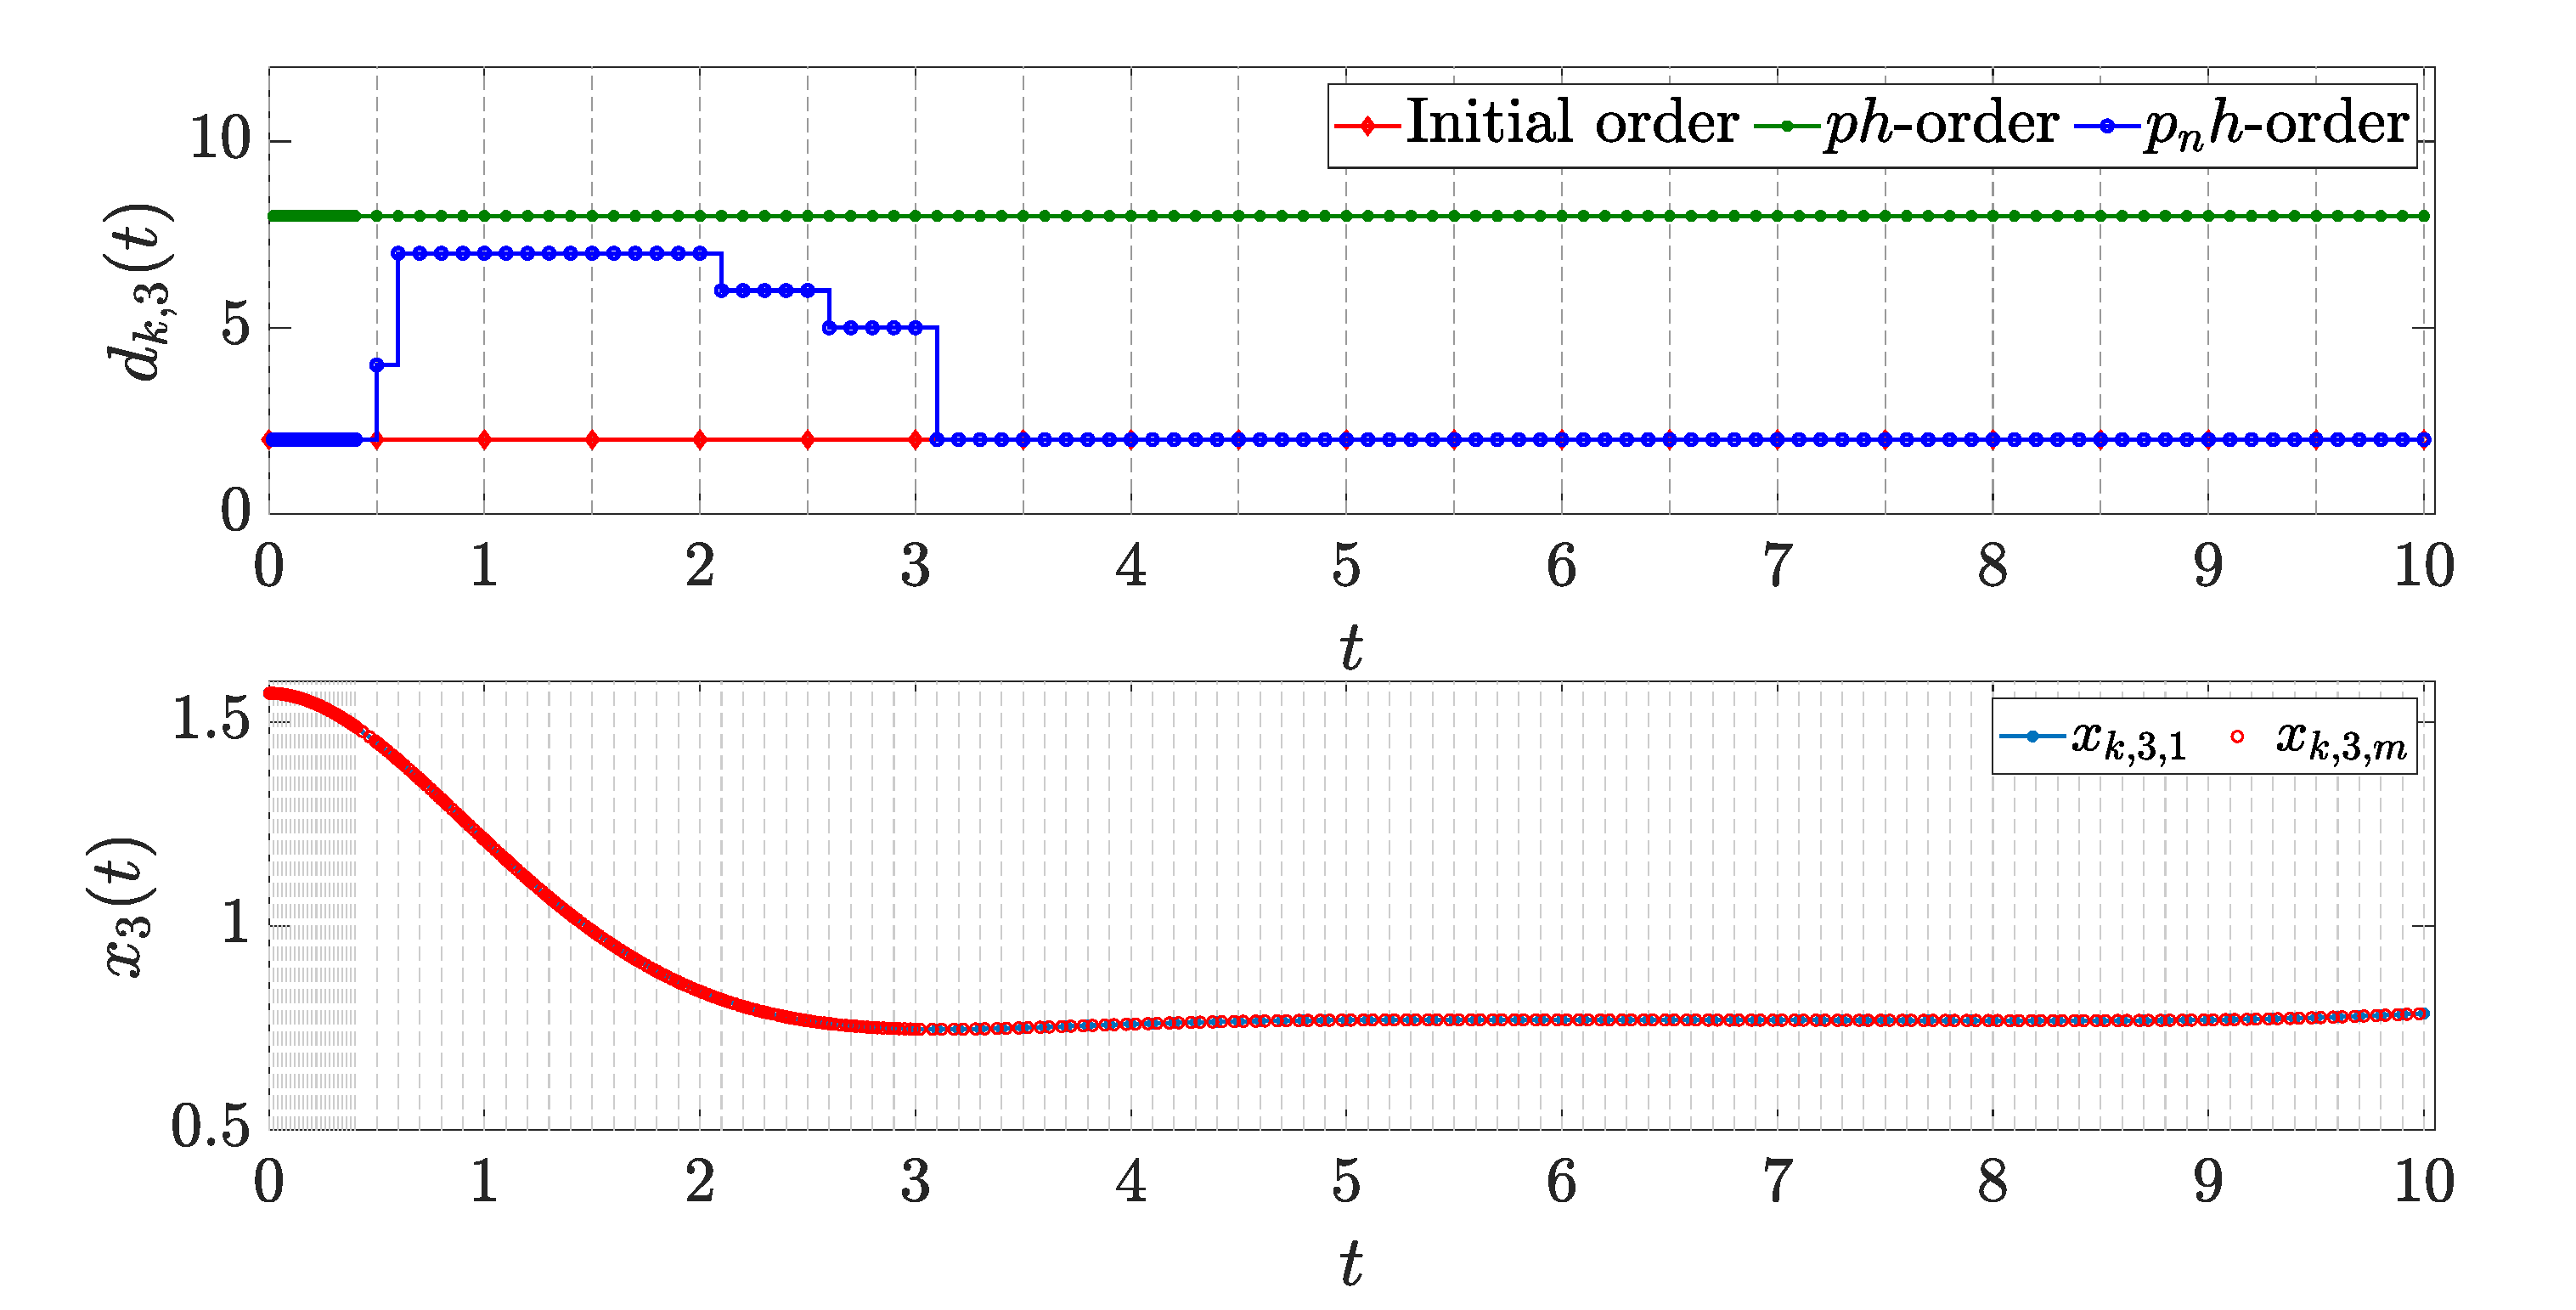
\includegraphics[trim={1cm 0.1cm 2cm 1.05cm},clip,width=1.\columnwidth]{Img/pnh2_disk2}
	\caption{EXAMPLE 2: (TOP) POLYNOMIAL DEGREE OF THIRD STATE ($x_{3}$) FOR THE INITIAL MESH (RED) FOR $\pnh$ ALGORITHM (BLUE) AND FOR $ph$ ALGORITHM (GREEN), (BOTTOM)
	OPTIMAL $x_3$ PROFILE OBTAINED WITH $\pnh$.}
	\label{fig:pnh2disk}
\end{figure}
%%%%%%%%%%%%%%
The advantages of the $\pnh$ method with respect to the $ph$ one, are summarized in Table~\ref{tab:tabledisk}. Is is interesting to note that, even if $\pnh$ method needs an extra iteration, it maintains a total time equal to the $ph$ method. Furthermore, under the same $e_{\max}$, the number of variables involved in the last NLP (leading to the most accurate solution) of $\pnh$ are 25\% less than the original method. This represent a noteworthy reduction.

For what concerns the nodal deviations of the $\pnh$ and $ph$ solutions at nodal values, the maximum value is registered for $u_2$. Again, this difference is in the order of $10^{-6}$, which is absolutely negligible given the control signal $u_2$ in the order of $10^0$. Therefore, the two methods lead to equally accurate solutions.
\begin{table}[t]
	\caption{EXAMPLE 2: MESH REFINEMENT RESULTS FOR THE THREE DIFFERENT TYPE OF MESH (INITIAL MESH, $ph$ FINAL MESH AND $\pnh$ FINAL MESH)}
	\begin{center}
		\label{tab:tabledisk}
		\begin{tabular}{c c c c c c c}
			& & \\ % put some space after the caption
			\hline
			\emph{Mesh} & \emph{Vars} & \emph{Soln. time} & \emph{Iter} & \emph{Tot. time} & $e_\text{max}$ \\
			\hline
			\emph{Initial} & 400 & 0.643 s & / & / &  $3.6\cdot 10^{-2}$\\
			$ph$  & 6496 & 61.6 s & 4 & 287.7 s & $9.8\cdot 10^{-4}$ \\
			$\pnh$ & 4810 & 32.4 s & 5 & 287.1 s & $9.8\cdot 10^{-4}$ \\
			\hline
		\end{tabular}
	\end{center}
\end{table}
%\newline
%\newline
%%%%%%%%%%%%%%%%%%%%%%%%%%%%%%%%%%%%%%%%%%%%%%%%%%%%%%%%%%%%%%%%%%%%%%
\subsection*{Example 3: Free-Flying Robot}
As the last example, we consider to optimally control the attitude of a 2D free-flying robot endowed with a propulsion system. This problem is taken from reference~\cite{Betts:book:2010}, with a modified cost function. Analytically, it can be framed as follows
\begin{subequations}\label{eq:free}
	\begin{align}
	\underset{X \in \mathbb{R}^{6}, \, U \in \mathbb{R}^{2}}{\text{minimize}}\hspace{8mm}
	&J = \int_{0}^{T}(u_{1}^{2} +  u_{2}^{2})\,dt  \label{eq:freecost}\\
	\text{subject to} \hspace{8mm}
	& \dot{x}_1 = x_4 \hspace{28mm} t \in[0,T] \label{eq:freedyn1}\\
	& \dot{x}_2 = x_5 \hspace{28mm} t \in[0,T] \label{eq:freedyn2}\\
	& \dot{x}_3 = x_6\hspace{28mm} t \in[0,T] \label{eq:freedyn3}\\
	& \dot{x}_4 = (u_1 + u_2)\cos(x_3)\hspace{7.5mm} t \in[0,T] \label{eq:freedyn4}\\
	& \dot{x}_5 = (u_1 + u_2)\sin(x_3)\hspace{8mm} t \in[0,T] \label{eq:freedyn5}\\
	& \dot{x}_6 = \alpha u_1 - \beta u_2\hspace{16mm} t \in[0,T] \label{eq:freedyn6}\\
	&X(0) = [-10, -10, \pi/2, 0, 0, 0]\\
	&X(T) = [0, 0, 0, 0, 0, 0], \label{eq:freefinal1}		
	\end{align}
\end{subequations}
where $x_1$ and $x_2$ are the inertial coordinates of the center of gravity, $x_4$ and $x_5$ are the corresponding velocities, and $x_3$ and $x_6$ are the thrust direction and the angular velocity, respectively. The thrust from the two engines, denoted by $u_1$ and $u_2$, serve as the control variables. Finally, $T = 12$ s and $\alpha = \beta = 1$.
%%%%%%%%%%%%%
\begin{figure}[t]
	\centering
	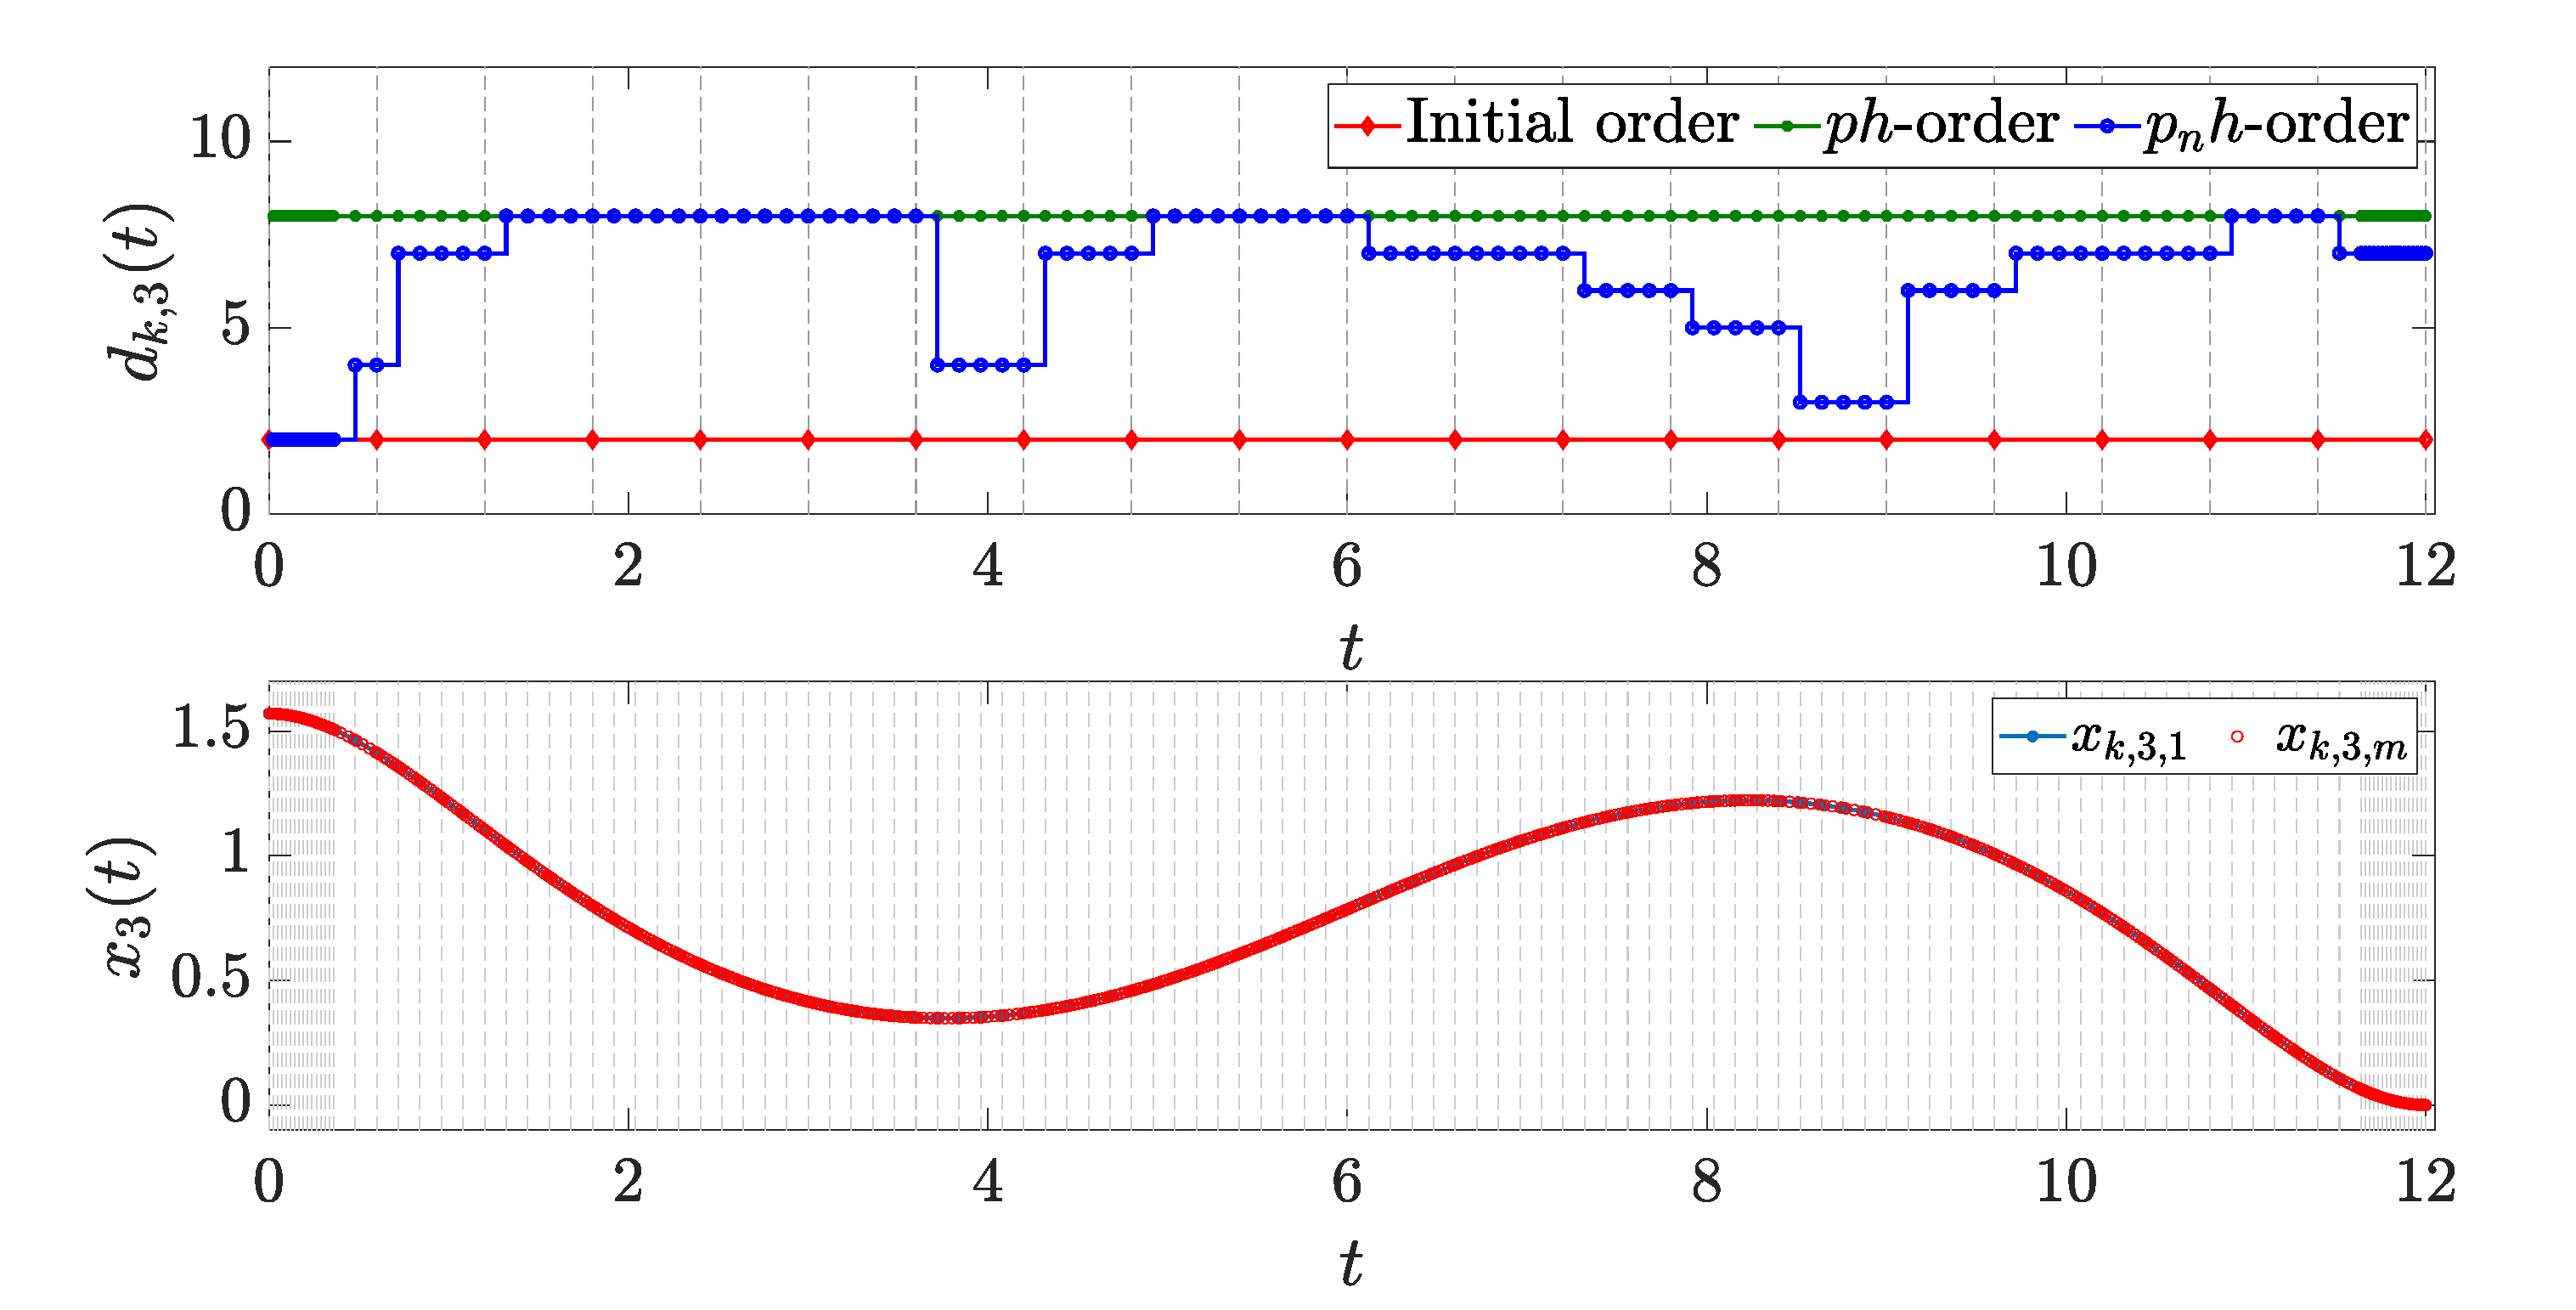
\includegraphics[trim={1cm 0.1cm 2cm 1.05cm},clip,width=1.\linewidth]{Img/pnh1_free}
	\caption{EXAMPLE 3: (TOP) POLYNOMIAL DEGREE OF $x_{3}$ FOR THE INITIAL MESH (RED), FOR $\pnh$ ALGORITHM (BLUE) AND FOR $ph$ ALGORITHM (GREEN), (BOTTOM) OPTIMAL $x_3$ PROFILE OBTAINED WITH $\pnh$.}
	\label{fig:pnh1free}
\end{figure}
%%%%%%%%%%%%%%%%

Due to space constraints, in Figure~\ref{fig:pnh1free}, only the results for the thrust direction $x_3$ are depicted. Clearly, the final order required by $\pnh$ method is very different from the $ph$ counterpart. Furthermore, considering the state profile, it is worth observing that the $h$-refinement strategy is favored at the beginning and at the end of the trajectory.

The advantages of the $\pnh$ method with to the $ph$ one, are shown in Table~\ref{tab:tablefree}. Under the same practical accuracy, $\pnh$ method guarantees about $20\%$ less NLP variables involved and about $27\%$ reduction in total time with respect to the $ph$ counterpart.

As for nodal differences between $\pnh$ and $ph$ solutions, the maximum value is reached for state $x_1$. A maximum difference in the order of $10^{-7}$ reveals that it is practically negligible given a state $x_1$ in the order of $10^0$. Hence, the two methods lead to the same solution.
\begin{table}[t]
	\caption{EXAMPLE 3: MESH REFINEMENT RESULTS FOR THE THREE DIFFERENT TYPE OF MESH (INITIAL MESH, $ph$ FINAL MESH AND $\pnh$ FINAL MESH)}
	\begin{center}
		\label{tab:tablefree}
		\begin{tabular}{c c c c c c c}
			& & \\ % put some space after the caption
			\hline
			\emph{Mesh} & \emph{Vars} & \emph{Soln. time} & \emph{Iter} & \emph{Tot. time} & $e_\text{max}$ \\
			\hline
			\emph{Initial} & 400 & 0.643 s & / & / &  $3.7 \cdot 10^{-2}$\\
			$ph$  & 6944 & 79.8 s & 4 & 367.1 s & $8.9\cdot 10^{-4}$ \\
			$\pnh$ & 5550 & 63.6 s & 4 & 271.3 s & $9.2\cdot 10^{-4}$ \\
			\hline
		\end{tabular}
	\end{center}
\end{table}


%\cite{latex, goosens} 